\documentclass[12pt, paper=a4]{article}
\usepackage[utf8]{inputenc}
\usepackage[german]{babel}
\usepackage{mathrsfs}
\usepackage{amsmath}
\usepackage{amssymb}
\usepackage{listings}
\usepackage{graphicx}
\usepackage{fancyhdr}

\setlength{\parindent}{0pt}

\author{Mareike G\"ottsch, 6695217, Gruppe 2\\Paul H\"olzen, 6673477, Gruppe 1\\Sven Schmidt, 6217064, Gruppe 1}

\title{FGI 2 Hausaufgaben 8}

\rhead{M. G\"ottsch, G-2; P. H\"olzen, G-1; S. Schmidt, G-1}
\pagestyle{fancy}
\begin{document}
\maketitle

\section*{Aufgabe 8.3}
\subsection*{1.}



\section*{Aufgabe 8.4}

Zun\"achst wurde aus dem Netz der Erreichbarkeitsgraph erstellt:

\begin{figure}[h!]
\centering
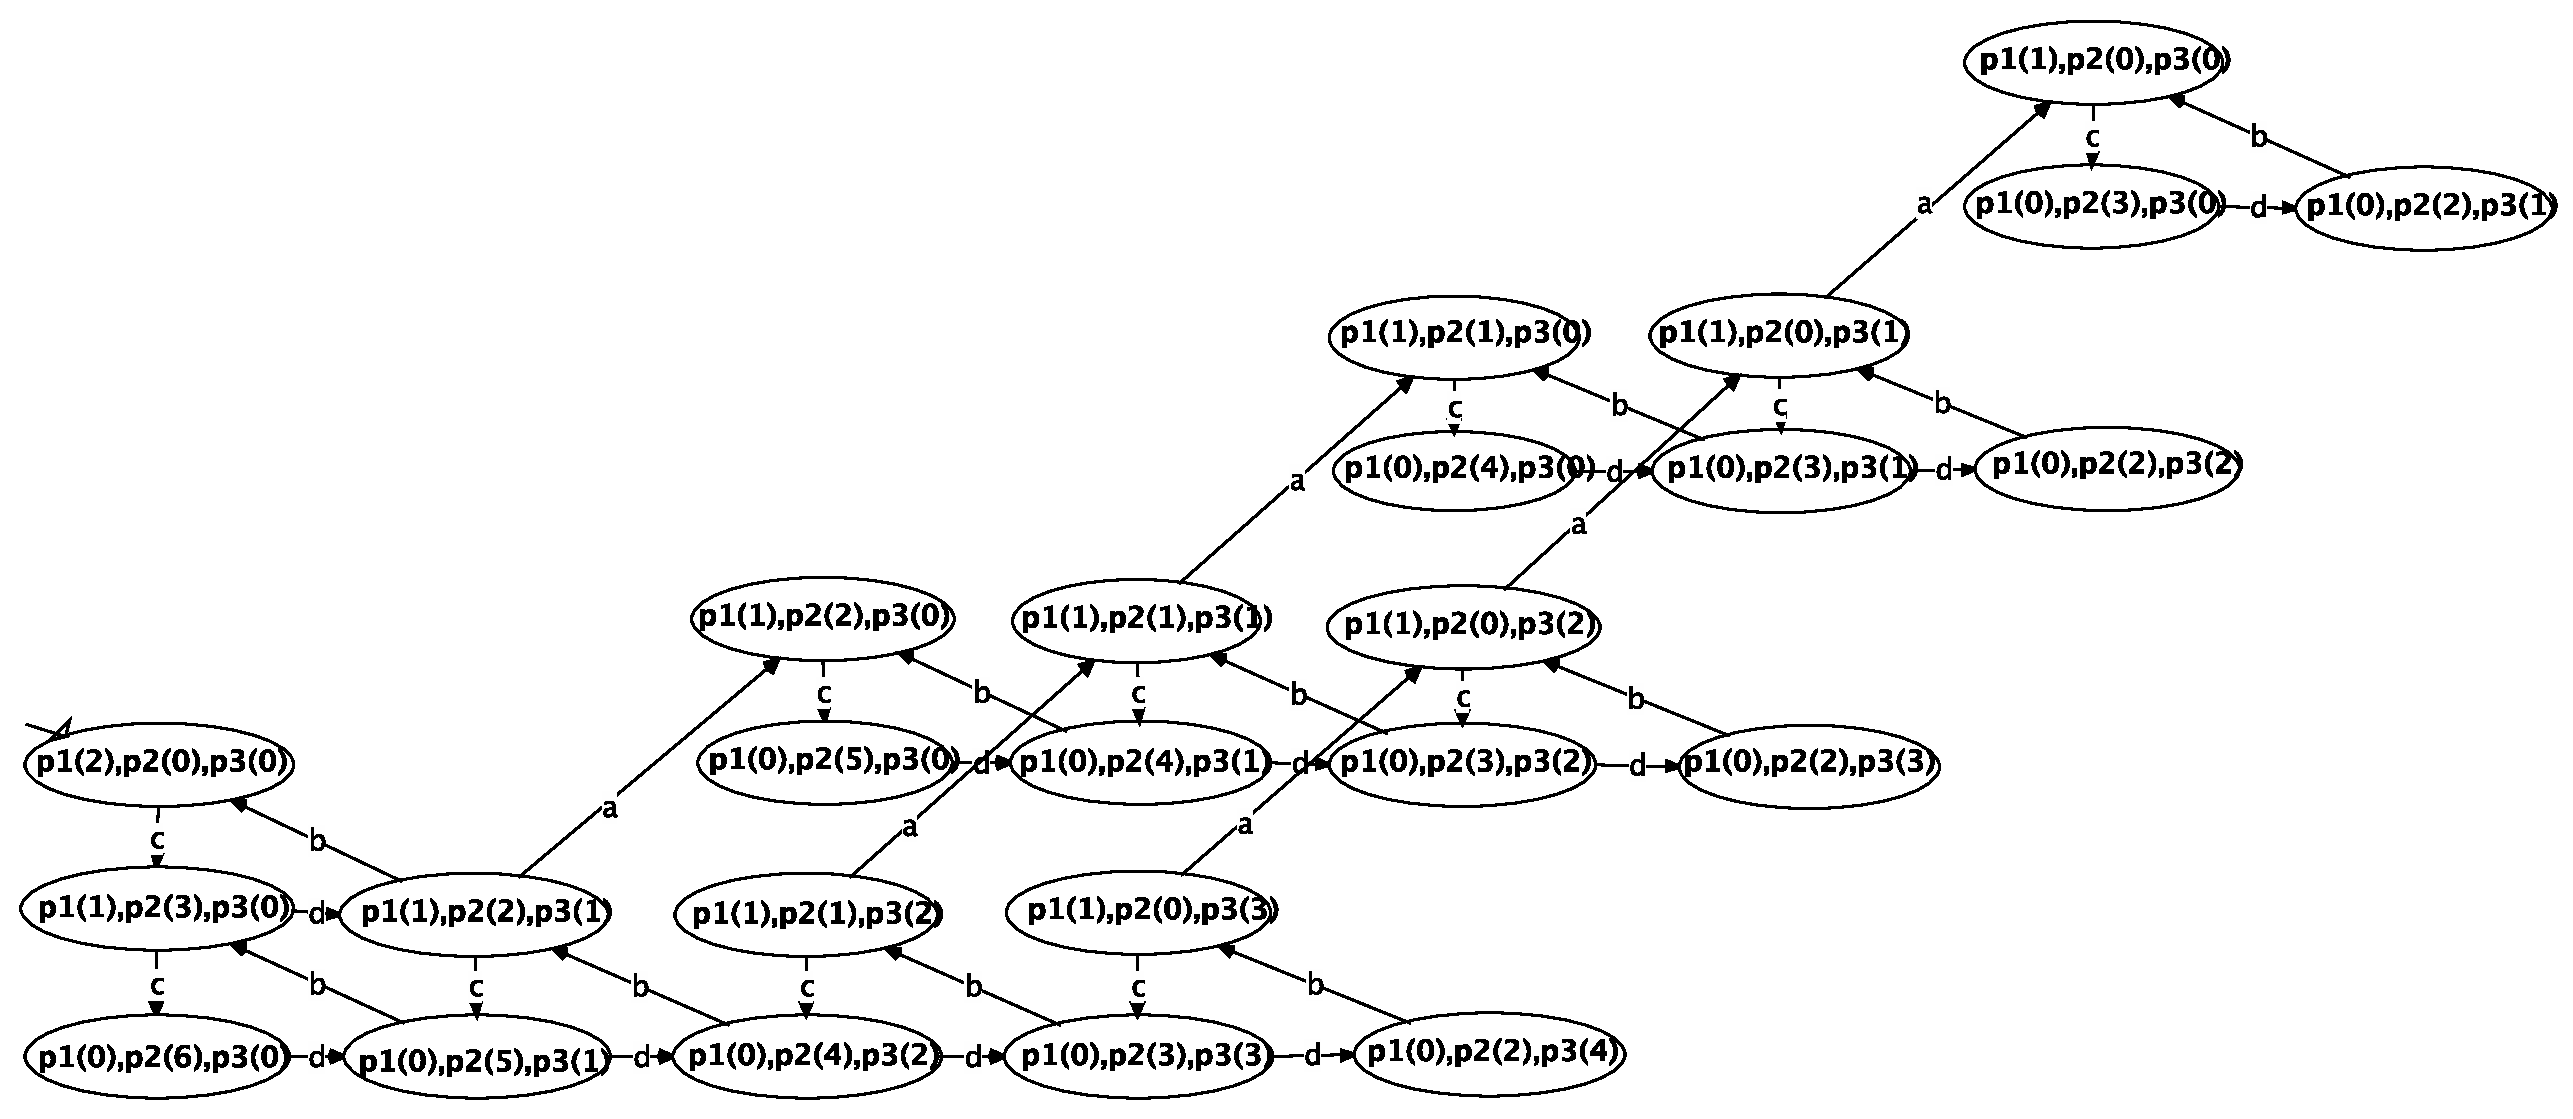
\includegraphics[scale=0.35]{8_4errg.pdf}
\caption{Erreichbarkeitsgraph von N8.4}
\end{figure}

Davon ausgehend wurden die starken Zusammenhangskomponenten \( C_1, C_2, C_3 \) und \( C_4 \) gebildet:

\begin{figure}[h!]
\centering
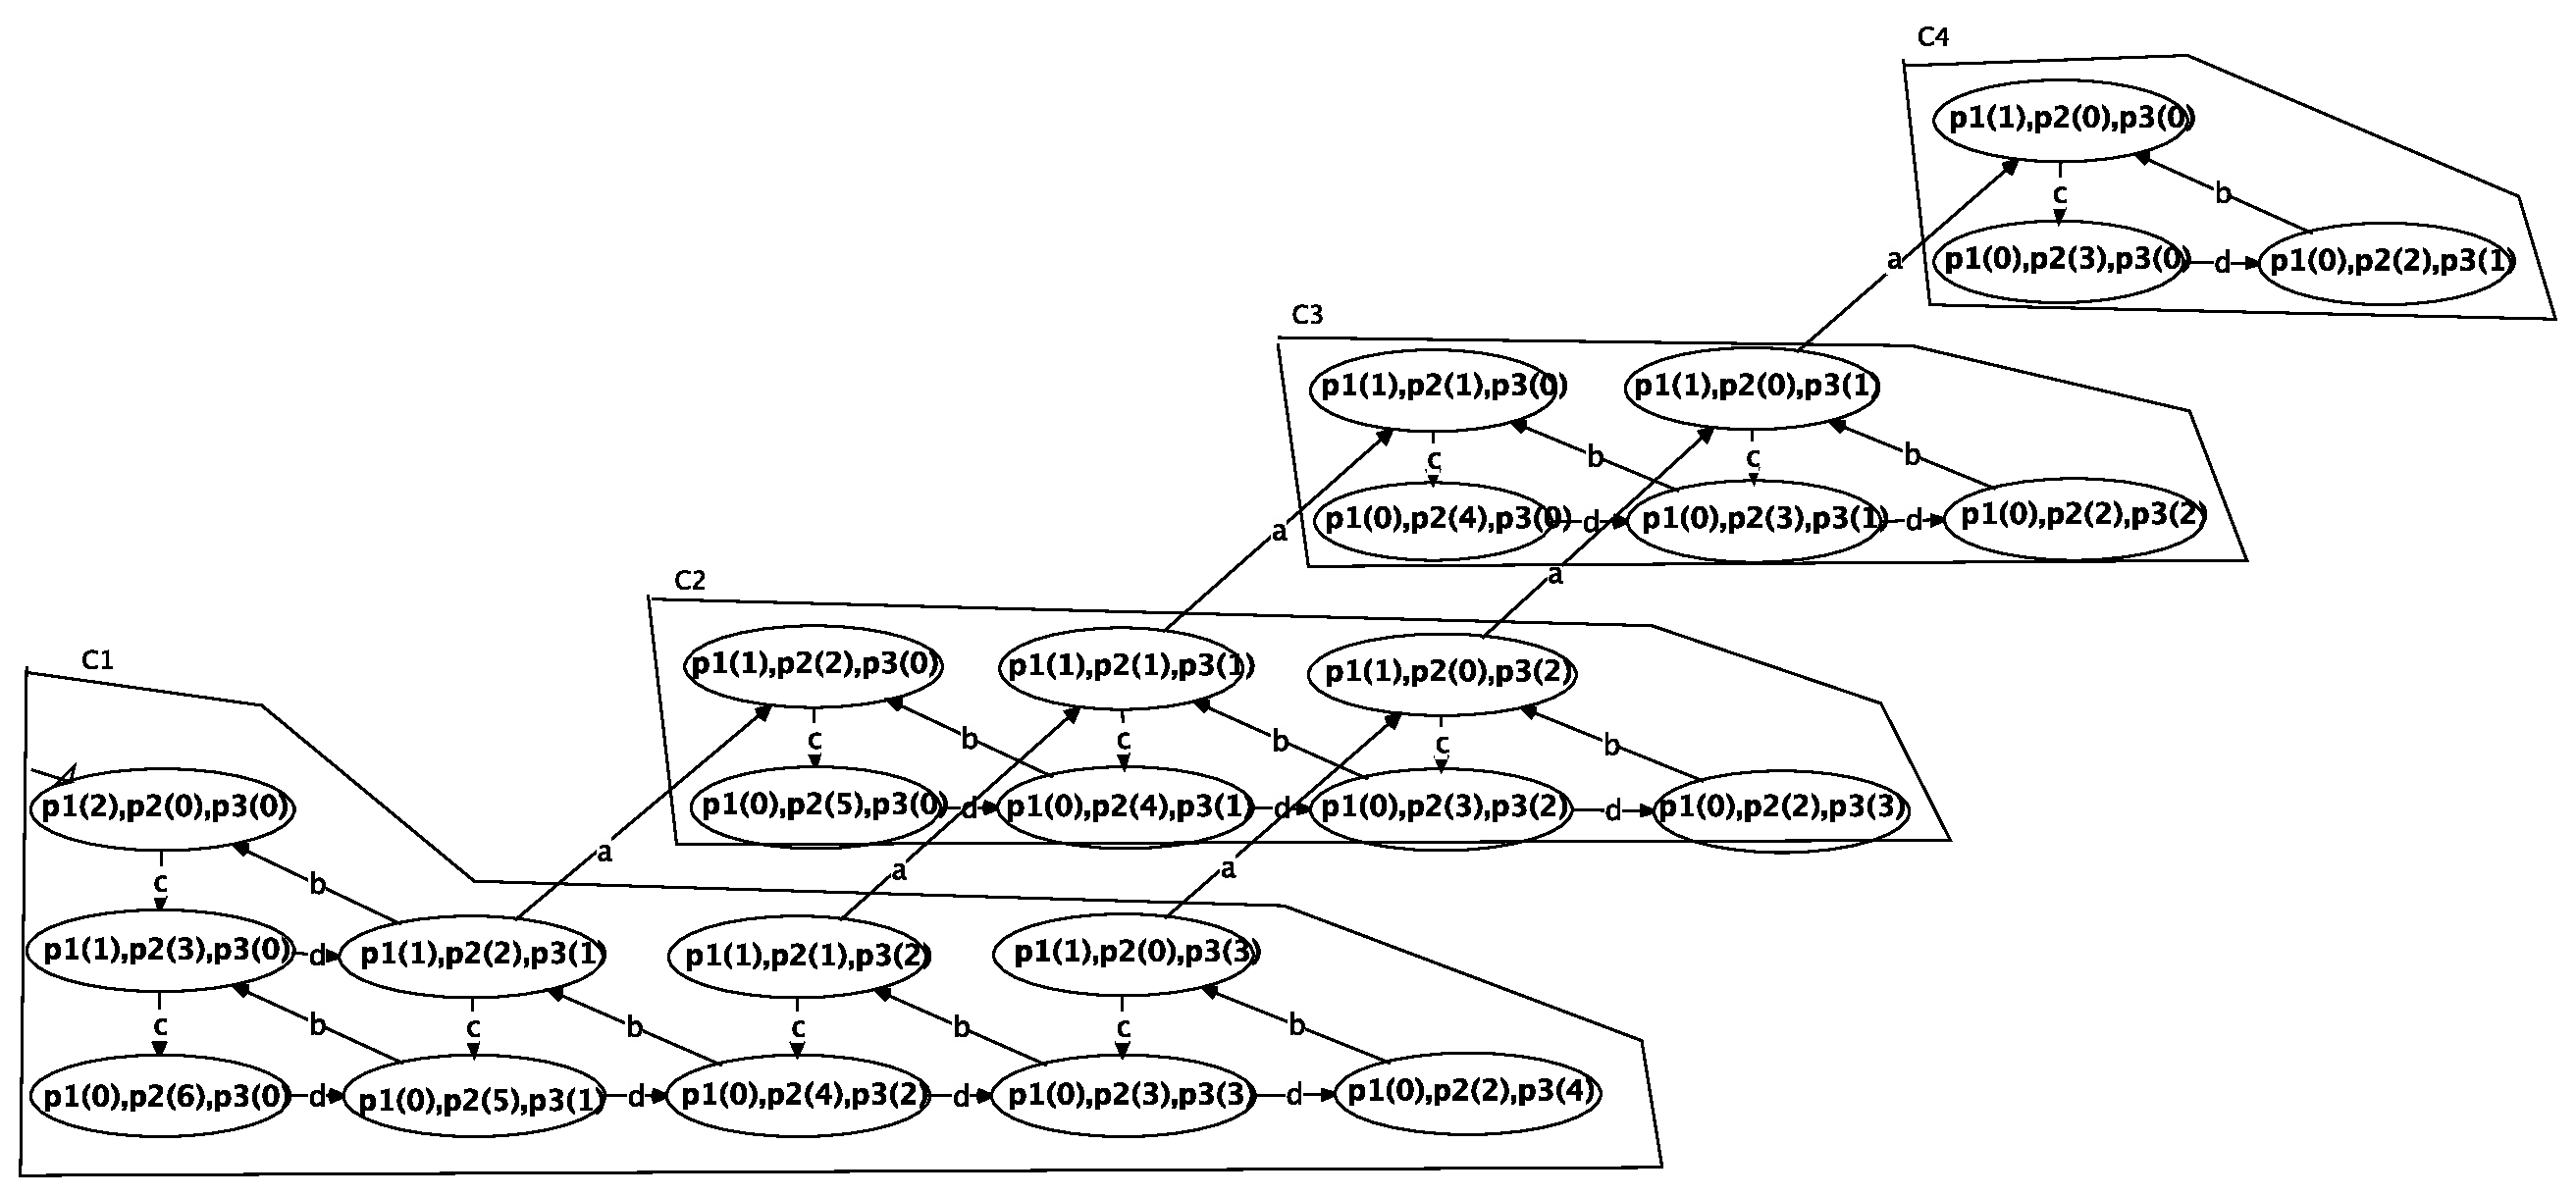
\includegraphics[scale=0.35]{8_4SZK.pdf}
\caption{SZKs von N8.4}
\end{figure}

Anschlie{\ss}end wurde daraus der reduzierte Graph \(RG^c(\mathcal{N},m_0)\) erstellt.\\
Dabei ist \(V_c = \{C_1,C_2,C_3,C_4\}\) die Knotenmenge, welche von den SZKs gebildet wird und\\
\(E_c = \{(C_1,a,C_2), (C_2,a,C_3), (C_3,a,C_4)\}\) die Kantenmenge.

\begin{figure}[h!]
\centering
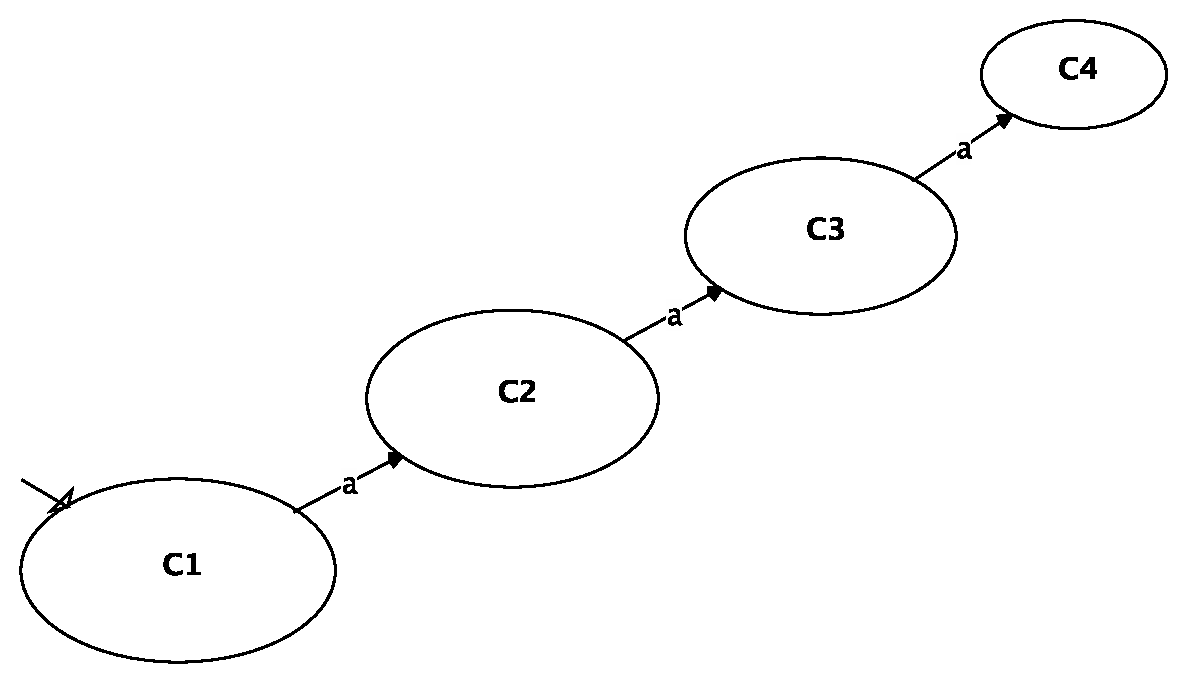
\includegraphics[scale=0.4]{8_4RGc.pdf}
\caption{reduzierter Graph von N8.4}
\end{figure}

Von den Zusammenhangskomponenten ist \(C_4\) terminal, d.h. \(F=\{C_4\}\).

\section*{Aufgabe 8.5}

\end{document}
